\chapter{Entwicklung einer real-time Query Anwendung zur Beschleunigung von Userprofilqueries}
In der bestehenden Betriebsanwendung werden Nutzer zum Zweck von Umfrageteilnahmen verwaltet. Nutzer pflegen Profilangaben, um dann passgenau zu Umfragen eingeladen zu werden.
Ein wesentlicher Bestandteil der Anwendung bildet das Abfragen eben dieser Nutzerprofildaten. Um für Umfragen passgenau Teilnehmer auszuwählen, gibt es in der Profildatenbank, die knapp 400.000 Nutzer umfasst, 176 Profilfelder. Diese können in allen denkbaren Kombinationen abgefragt werden. Die besteheden Datenbankabfragen geschehen aufgrund ihrer langen Laufzeit asynchron. Hier soll eine neue Echtzeitschnittstelle geschaffen werden.

\section{Real-time Anforderungen erzwingen eine neue Entwicklung}
Da das Finden von Umfrageteilnehmern und demnach das Abfragen der Profilfelder einen wesentlichen Kern der Betriebsanwendung bildet, besteht dieser Teil der Anwendung mit am längsten. In den fast 3 1/2 Jahren ist sowohl die Anzahl der Nutzer, also auch die Anzahl der Profilfelder enorm gewachsen, weitaus mehr als initial erwartet. Im Laufe der Zeit stellte sich heraus, das die gewählte Datenbanktechnologie MongoDB, die gewählte Datenstruktur und die Art wie gequeried wird, nicht optimal und daher nicht schnell genug sind. Da das Abfragen der Profilfelder wesentlichster Bestandteil des Kerngeschäfts ist und die Defizite die Situation mit wachsender Nutzer- und Kundenzahl nur verschärfen, wurde deutlich, dass eine Überarbeitung der bestehenden Strukturen notwendig ist.

Das Ziel der Neuentwicklung ist vor Allem, die Profilqueries zu beschleunigen, ohne dadurch an andere Stellen Performance einzubüßen. Da viele Queries, besonders auf solche Felder, die nicht durch einen Index abgedeckt sind, sehr langsam sind, soll hier eine signifikante Zeitersparnis erreicht werden. Zum Anderen soll aber gleichzeitig auch die Struktur des Codes verbessert werden. Fast die gesamte Anwendung befindet sich zur Zeit in einem Repository. Die Strukturen sind zum Teil sehr vermischt und Abhänigkeiten bestehen auch dort, wo keine bestehen sollten. Der neu entworfene Code soll klare Strukturen und klare Schnittstellen besitzen.

\section{Majestic Monolith vs Minimal Microservice}
Um die genannten Probleme zu lösen, können jedoch verschiedene Lösungsansätze zur Optimiertung verfolgt werden. Zum Einen kann eine neue Datenbanktechnologie mit optimiertem Schema gewählt werden. Zum Anderen kann der Code auf Geschwindigkeit optimiert oder komplett neu geschrieben werden.
Da die in der Anwendung eingesetzte Datenbank MongoDB noch für weitere Teile der Anwendung genutzt wird, kann sie nicht komplett ausgetauscht werden. Da es sich jedoch zur Optimierung sowohl anbietet eine neue Datenbanktechnologie einzusetzen, als auch den Code zu verbessern, bietet sich die Entwicklung eines separaten Microservices an. Hier kann eine optimierte Datenbanktechnologie eingesetzt werden ohne die bestehende Anwendung um weitere Strukturen und somit Komplexitäten zu ergänzen. Der Code kann restrukturiert und verbessert werden, in dem klarere und eindeutigere Strukturen und Aufteilungen geschaffen werden

Des Weiteren erlaubt es ein separater Service passgenauere Skalierung. Durch dynamisches Hosting kann so also nicht nur die inhärente Performance von Code und Datenbank verbessert werden, sondern die reale auch dadurch, Ressourcen optimiert einzusetzen.
Eine neue Datenbanktechnologie und neuer Code bieten sich zur Auslagerung in einen Microservice an. So wird der bestehende Code umgeschrieben um eine neue, separate Schnittstelle zu verwenden und im Funktionsumfang reduziert. Code zum Zweck der Nutzerabfragen findet sich in einer sauber getrennten Codebase und kann leicht gepflegt werden.

\section{Mit dem Strangler Pattern vom Monolithen zur Microservice Architektur}
Da die aktuelle Arbeitslage, die vorhandenen Entwickler und die Größe der Anwendung es nicht zulassen, diese direkt komplett zu überarbeiten, wird hier die Architektur mit Hilfe des Strangler Patterns Schritt für Schritt verändert.
Der Name des Stangler Patterns ist aus einer Analogie zur Botanik entstanden. Hierbei wurde von Fowler\cite[][]{Fowler:Strangler} der Vergleich zur Würgefeige (engl. Strangler Fig) gezogen. Diese wächst von den Ästen an einem Wirtsbaum herab, bis sie den Boden erreicht. Nach und nach wird der Wirtsbaum immer weiter umschlossen, bis er schließlich abstirbt.
Ähnlich kann bei der Softwareentwicklung zum Ersetzen einer alten Anwendung vorgegangen werden. An bestimmten, sich eignenden Stellen, wird begonnen Teile der bestehenden Anwendung zu ersetzen. Neuer Code wird geschaffen und nach und nach die Last auf die neue Teilanwendung geleitet.
Dieses Vorgehen bietet viele Vorteile gegenüber dem kompletten Austausch einer Altanwendung. Die neue Anwendung kann Stück für Stück mit agilen Methoden und häufigen Deploys entwickelt und im Produktionsbetrieb betrachtet werden. Die neu entstehende Anwendung kann hierbei nach Belieben angepasst werden, um die Altanwendung mit möglichst geringem Risiko zu Ersetzen.
Zur Umsetzung dieses Ersetzens gibt es viele Wege. Zwei ebenfalls von Fowler vorgebrachte Strategien sind Asset Capture\cite[][]{Fowler:Capture} und EventInterception\cite[][]{Fowler:Interception}.
Beim AssetCapture geht es vor Allem darum, solche Assets zu identifizieren, die sich leicht in die neue Teilanwendung migrieren lassen. Dies können bestimmte Tabellen in der Datenbank sein. Im Fall der zu entwickelnden Anwendung sind dies die Nutzerprofile.
EventInterception geht mit AssetCapture Hand in Hand. Hierbei müssen alle Events auf die ausgelagerten Assets, also zum Beispiel das Abfragen von Profilen und das Anlegen neuer Profile, abgefangen und umgeleitet werden.
So wird sichergestellt, dass die alten Ressourcen nicht mehr aktualisiert werden und es nicht zu Inkonsitenzen im Datenbestand kommt.
Um die bestehende Betriebsanwendung auf Microservices umzustellen, wird hier ähnlich vorgegangen. Aus gegebenem Anlass wird der Query-Microservice als erster Strangler entwickelt. Die Nutzerprofile eignen sich gut um sie in eine neue Datenbank zu migrieren und in diesem Schritt gleich zu optimieren. Ein neuer Service verwaltet hierzu den Zugriff auf die Daten. Die bestehenden Events zum Abfragen von Nutzerprofildaten werden auf den neuen Service umgestellt. Hier wird eine Schnittstelle geschaffen, die sowohl Zugriff auf den neuen Service, als auch auf die alte Datenbank zulässt. Wird eine neue Anwendung mit Userschnittstelle geschaffen, bietet es sich an, einfach nach und nach mehr der Seitenzugriffe auf das neue System umzuleiten. Zum Einen auf Makroebene, also Feature für Feature ablösen, aber auch auf Mikroebene bei Ersetzen eines Features. So können Fehler im neuen System minimiert werden und die Belastbarkeit des Systems sichergestelllt werden.
\begin{figure}[h]
    \caption{Load Balancer zur Strangulation Verteilung \cite{Hammant:Strangler}}
    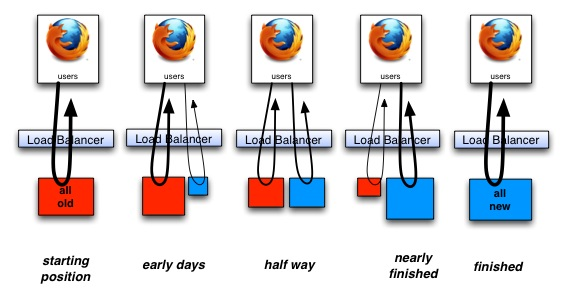
\includegraphics[width=\textwidth]{strangulation}
\end{figure}

Da der entwickelte Microservice keine Schnittstelle zum Web, sondern nur zum bereits bestehenden Monolithen hat, beschloss ich hier mit dem dem Strangler Pattern ähnlichen Prinzip der Feature Toggles\cite{fowler:featuretoggle} zu arbeiten. Statt mit einem Load Balancer, wird mit Hilfe des Ruby Flipper Gems\cite{flipper} nach und nach mehr Last auf den neu entstehenden Service zu verteilt.~\cite[vgl.][]{Hammant:Strangler}
Feature Toggles zeichnen sich dadurch aus, das über einen ``Schalter'' im Code gesteuert wird ob Requests zum neuen oder zum alten Feature geleitet werden. Beim Flipper Gem wird das Feature hier anhand einer \textit{Flag} in der Datenbank nur für bestimmte Nutzer aktiviert. So können beispielsweise für bestimmte Nutzer, zum Beispiel zunächst nur der Entwickler des neuen Features, der neue Dienst aktiviert werden, während alle anderen Nutzer noch den alten Service nutzen können. Dies dient zum Einen dem Testen des neuen Services auf Fehler, zum Anderen zur Evaluierung von dessen Performance.
Hierzu wird die zentrale Schnittstelle des QueryExecuters geschaffen. Die bestehende Schnittstelle zu MongoDB wird abstrahiert und um eine weitere, für den neuen Service ergänzt. Diese von den beiden Klassen gebotenen Schnittstellen sind identisch. Der QueryExecuter verteilt lediglich anhand der Flipper Logik an den neuen Microservice oder den bestehenden Code.

Eine Beispielimplementierung zur Verwendung des Flipper Gems lässt sich so abbilden:
\begin{lstlisting}[language=Ruby]
def query_layer
  if api_activated?
    @query_layer = prophet
  else
    @query_layer = mongo
  end
end

def api_activated?
  flipper[:prophet_api].enabled?(querying)
end
\end{lstlisting}
Der Query Executer fragt hier lediglich ab ob für das Querying Objekt in der Datenbank der Flipper für den neuen Microservice gesetzt ist. Ist dies der Fall, wird als Query Ebene der ProphetQuerier, ansonsten der MongoQuerier zurückgegeben.

Da die Nutzerprofile noch auf Seiten der Verwaltung der User selbst in der Hauptanwendung benötigt werden, werden hier jedoch nicht alle Events abgefangen. Lediglich die, die das Querien im Bereich des Samplings betreffen. Um Datenkonsitenz zu gewährleisten, werden einmal täglich alle veränderten Daten in den Microservice geupdated. Da sich Userdaten nicht häufig ändern und sich unter 100 Nutzer am Tag registrieren, reicht dies aus um ausreichend gute Query Ergebnisse zu erzielen.